\documentclass[a4paper,11pt]{article}
\usepackage[utf8]{inputenc}
\usepackage[ngerman]{babel}
\usepackage{amsmath}
\usepackage{amssymb}
\usepackage{geometry}
\usepackage{graphicx}
\usepackage{wrapfig}
\usepackage{multicol}
\usepackage{float}

\title{\vspace{-1.5cm} ALP III: Aufgabenblatt 12, Übungsgruppe 1.8 }
\author {Tobias Lohse, Marvin Kleinert, Anton Drewing}
\date{}
\geometry{top=2cm, left=3cm, right=3cm, bottom=2cm}

\begin{document}

\maketitle

\section*{Aufgabe 1}

\begin{multicols}{2}
\paragraph{Prim Algorithmus:}$\;$
\\  91 : Berlin - Frankfurt O
\\ 119 : Frankfurt O - Cottbus
\\ 138 : Cottbus - Dresden
\\ 220 : Dresden - Erfurt
\\ 180 : Erfurt - Fulda
\\  95 : Fulda - Frankfurt M
\\ 187 : Fulda - Bayreuth
\\ 239 : Bayreuth - Augsburg
\\ 117 : Augsburg - Garmisch P
\\ 240 : Frankfurt M - Aachen
\\ 123 : Aachen - Essen
\\ 249 : Essen - Bremen
\\ 110 : Bremen - Hamburg
\\ 262 : Frankfurt M - Freiburg

\paragraph{Kruskal Algorithmus:}$\;$
\\  91 : Berlin - Frankfurt O
\\  95 : Frankfurt M - Fulda
\\ 110 : Bremen - Hamburg
\\ 117 : Garmisch P - Augsburg
\\ 119 : Frankfurt O - Cottbus
\\ 123 : Essen - Aachen
\\ 138 : Cottbus - Dresden
\\ 180 : Erfurt - Fulda
\\ 187 : Fulda - Bayreuth
\\ 220 : Dresden - Erfurt
\\ 239 : Augsburg - Bayreuth
\\ 240 : Frankfurt M - Aachen
\\ 249 : Essen - Bremen
\\ 262 : Frankfurt M - Freiburg
\end{multicols}

\begin{figure}[h]
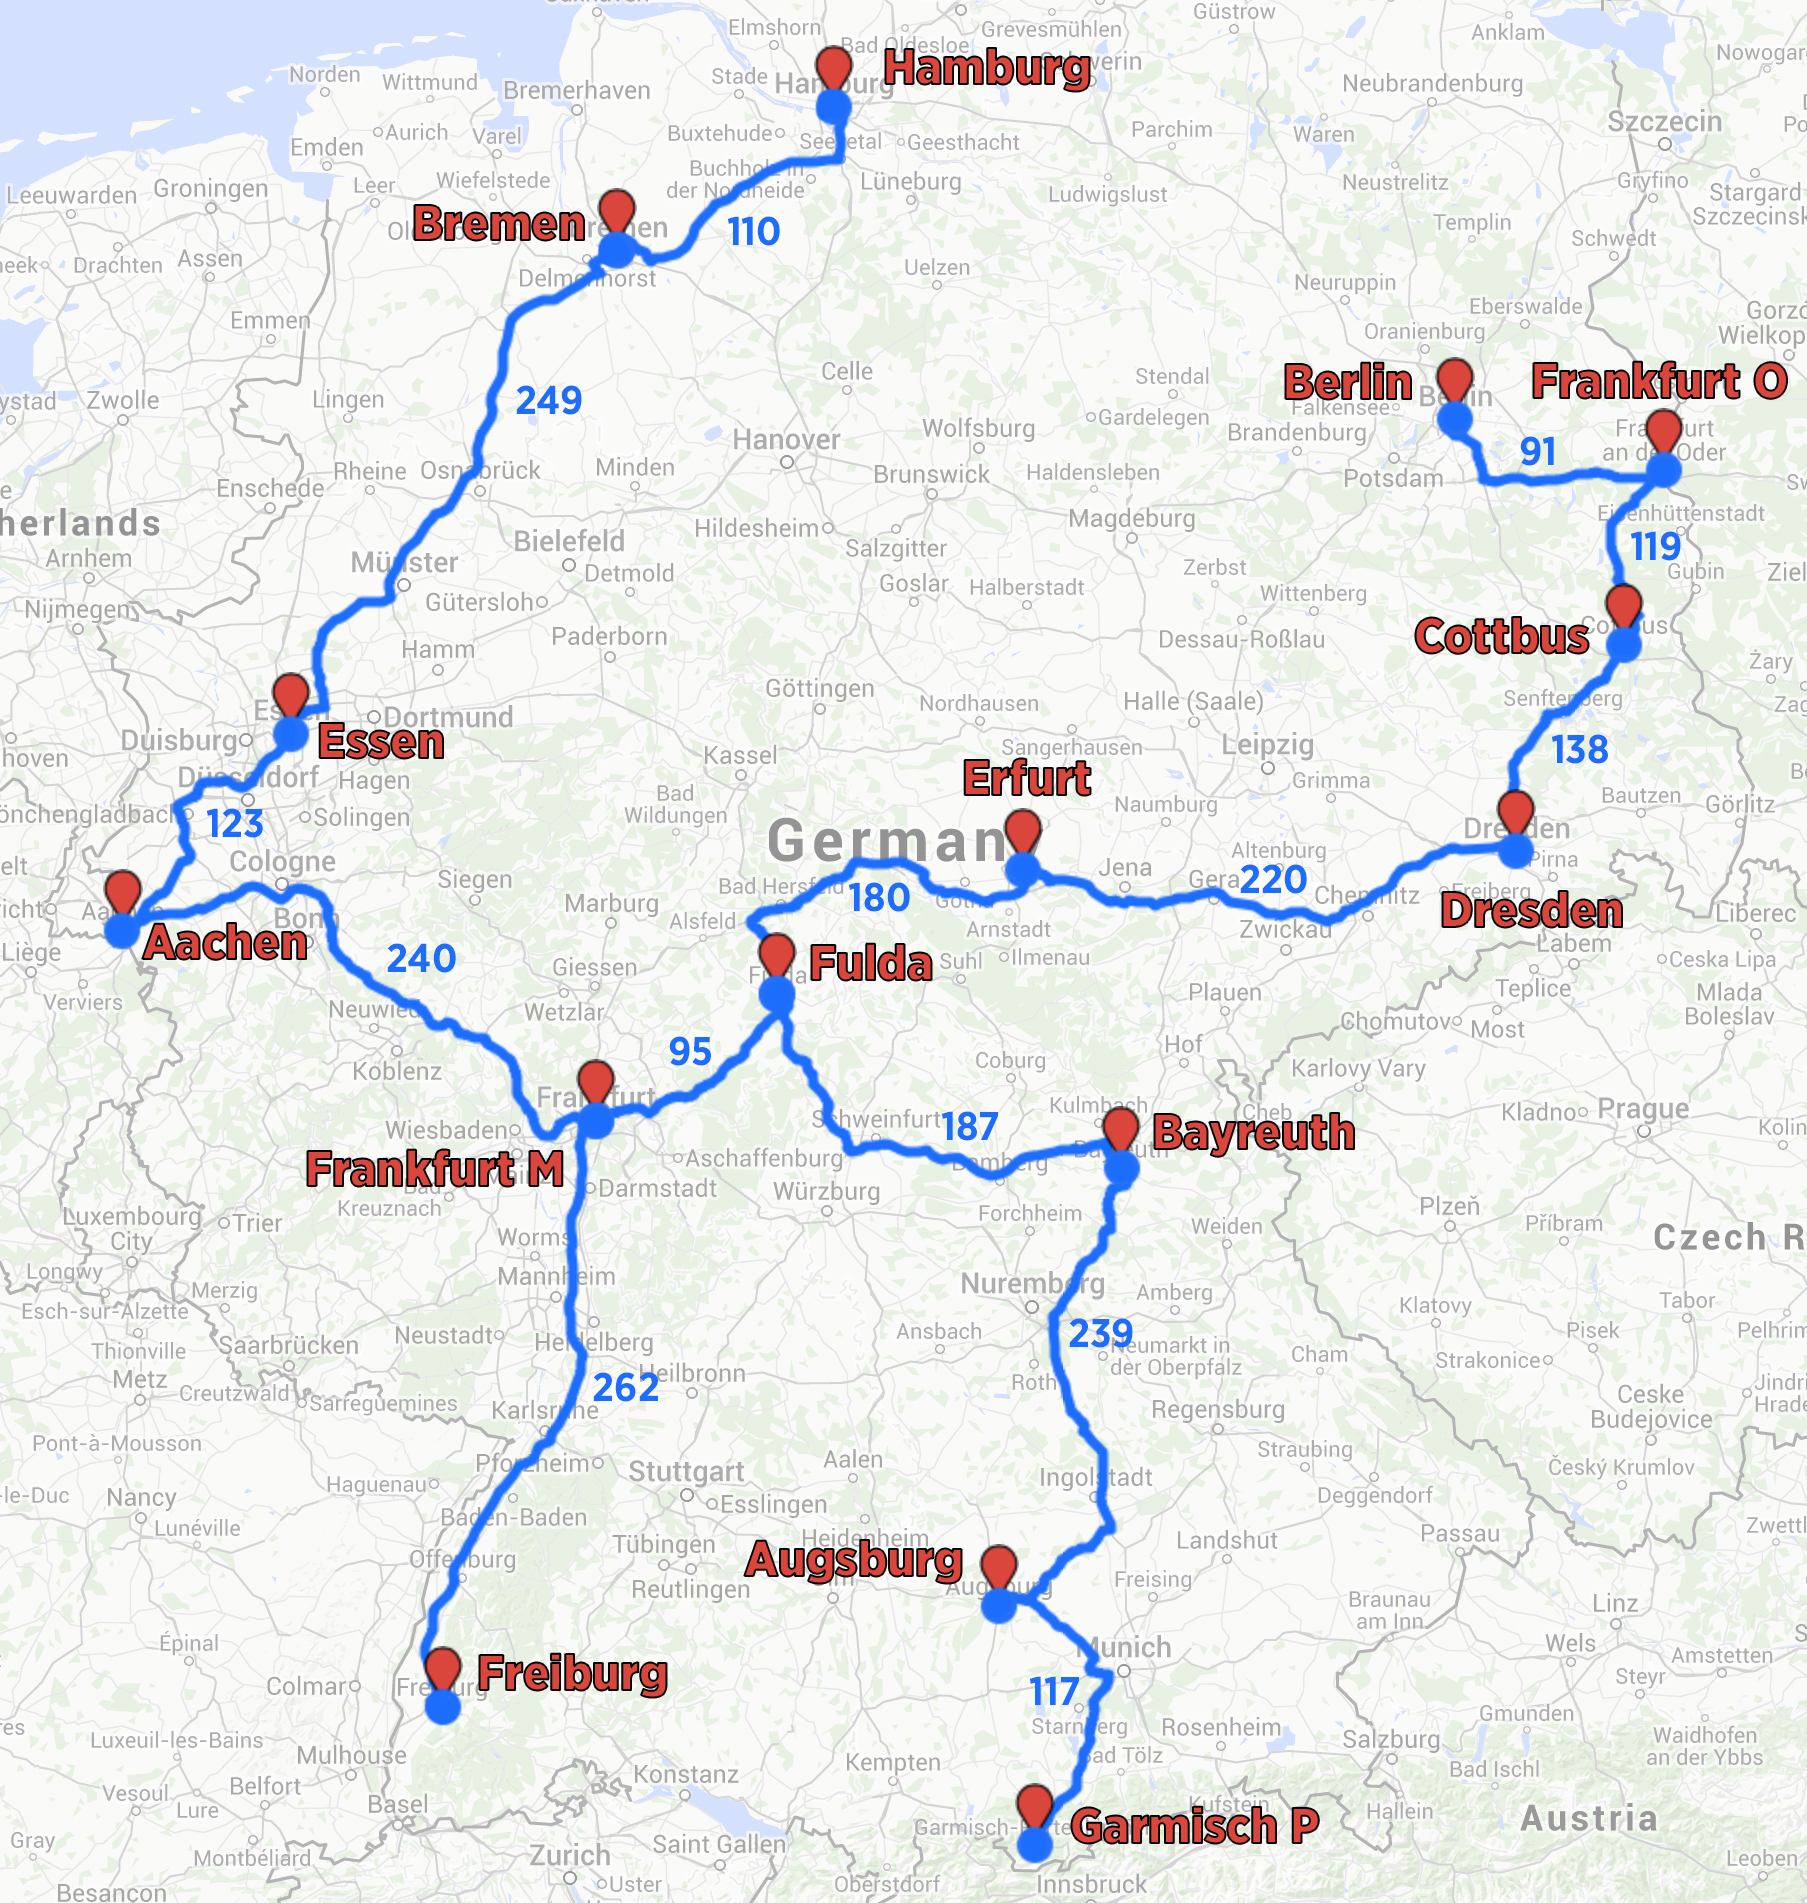
\includegraphics[width=0.89\textwidth]{a1/a1.jpg}
\end{figure}

\section*{Aufgabe 2}
Ein Graph $(V,E)$ mit injektiver Kostenfunktion $c: E \mapsto \mathbb{N}$ hat immer genau einen minimalen Spannbaum.

\paragraph{Beweise durch Widerspruch:}$\;$\\

Angenommen es gibt zwei minimale Spannbäume $S_1 = (V,E_1)$ und $S_2 = (V,E_2)$. Dann sortieren wir die Kanten $a_i \in E_1$ und $b_i \in E_2$ in den Spannbäumen in aufsteigender Reihenfolge nach ihren Kosten, also $\forall i<j : c(a_i)< c(a_j)$ und $\forall i<j : c(b_i)< c(b_j)$. Wir betrachten nun die Kanten $a_k \neq b_k$ mit kleinstem Index $k$, in der sich $E_1$ und $E_2$ unterscheiden. Aus der injektivität von $c$ folgt, dass $c(a_k) \neq c(b_k)$ und oBdA. nehmen wir an, dass $c(a_k) < c(b_k)$. \\

Nun konstruieren wir einen Graphen $(V,E')$ mit $E' = E_1 \cup \{a_k\}$. Da $E_1$ ein Spannbaum ist muss $E'$ nun einen Kreis $C$ haben, mit $a_k \in C$. Wir unterscheiden nun zwischen folgenden Fällen:

\paragraph{Fall 1:} $\exists e \in C: c(e) > c(a_k)$

Wenn wir nun $e \in C$ durch $a_k \in C$ austauschen in $E_2$, erhalten wir einen neuen Spannbaum $E_2' = E_2 \backslash \{e\} \cup \{a_k\}$. Da aber $c(a_k) < c(e)$ hat $E_2'$ geringere Kosten als $E_2$. Das steht im Widerspruch zur Annahme, dass $S_2$ ein minimaler Spannbaum ist.

\paragraph{Fall 2:} $\forall e \in C: c(e) < c(a_k)$

Da $a_k$ die Kante mit geringsten Kosten ist, in der sich $E_1$ und $E_2$ unterscheiden, müssen in diesem Fall all $e \in C$ auch in $E_1$ liegen. Damit gilt aber, dass $C \subseteq E_1$, der Spannbaum $S_1$ enthält also einen Kreis, das steht aber im Widerspruch dazu, dass es sich um einen Spannbaum handelt. \\

Es führt also zu einem Widerspruch, dass ein Graph mit injektiver Kostenfunktion zwei minimale Spannbäume hat, also kann ein solcher Graph nur einen einzigen eindeutigen Spannbaum haben.

\section*{Aufgabe 3}

Die UNION Operation hat eine Laufzeit von $\Theta(1)$, da nur ein Vergleich der Höhe der Bäume durchgeführt wird und dann von der Wurzel des niedrigeren Baums ein Pointer auf die Wurzel des höheren Baums hinzugefügt wird.\\

Die FIND Operation hat eine Laufzeit, die durch die Höhe $h$ der als Baum strukturierten Partition beschränkt ist, $O(h)$. Denn die Partitionene werden durch den Repräsentanten identifiziert, welcher die Wurzel des Baumes ist. FIND läuft also einfach zur Wurzel des Baumes, die höchstens $h$ weit weg sein kann. Enthält der Baum $k$ Knoten, so ist die Laufzeit von FIND also bei einem balancierten Baum im schlimmsten Fall $O(\log k)$.\\

Einen balancierten Baum erhält man durch $n$ UNION Operationen auf den $n$ ursprünglich einelementigen Partitionen, indem man immer Parweise 2 einelementige Partitionen zusammenfügt, dann 2 zweielementige Partitionen, dann 2 vierelementige Partitionen, usw. dabei nehmen wir oBdA. an, dass $\log n$ eine natürliche Zahl ist. Wir erhalten also mit $n$ UNION Operationen immer einen Baum mit Höhe $\log n$. Die $m$ finde Operationen brauchen dann also jeweils $\log n$.\\

Damit erhalten wir insgesamt eine Laufzeit von $\Omega(m \log n)$.








\end{document}